\subsection{Ordenamiento de Arreglos}
Se probaron arreglos de hasta $10^7$ elementos. En el siguiente gráfico se pueden ver los tiempos de ejecución registrados.

\begin{figure}[H]
    \centering
    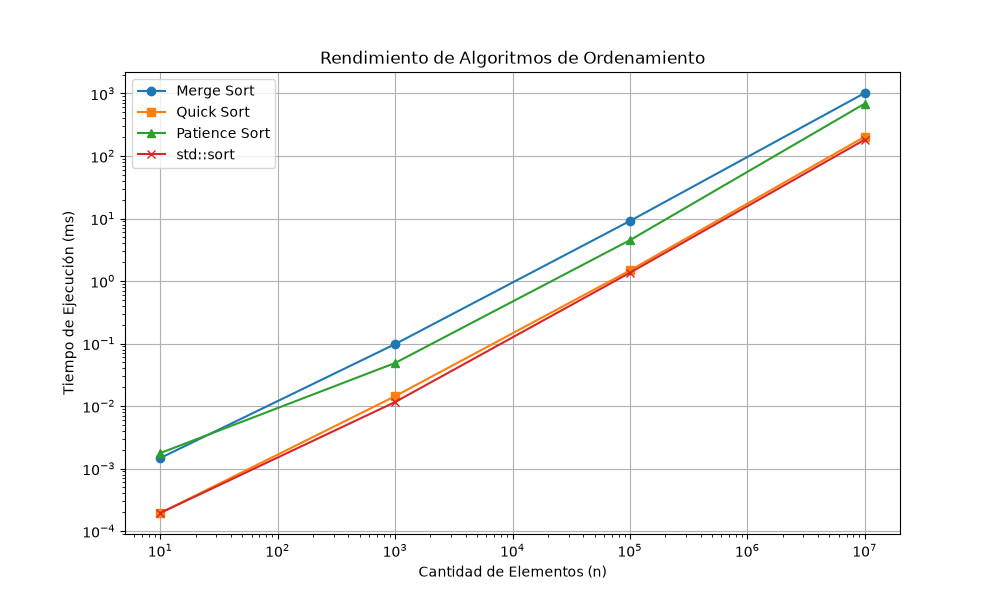
\includegraphics[width=0.8\textwidth]{../code/sorting/data/plots/ordenamiento_tiempo.png}
    \caption{Tiempos de ejecución para algoritmos de ordenamiento.}
    \label{fig:ordenamiento}
\end{figure}

Algo importante que notamos en las pruebas fue el comportamiento de Quick Sort. Al probarlo con arreglos gigantes y con muchos números repetidos, la versión clásica se fue a su peor caso de $O(n^2)$. Para evitar que el proceso se demorara una eternidad, implementamos una partición de 3 vías. Con eso, los tiempos volvieron a ser de $O(n \log n)$ y el algoritmo logró competir muy de cerca con el std::sort nativo de C++.

Adicionalmente, al contrastar estos resultados con los peores casos teóricos de cada algoritmo, el comportamiento varía drásticamente según la naturaleza de los datos. Algoritmos como Merge Sort y std::sort (que internamente implementa Introsort) mantienen un rendimiento altamente consistente de $O(n \log n)$ sin importar si el arreglo entra ordenado, invertido o desordenado. Sin embargo, Patience Sort es extremadamente sensible a la distribución inicial: frente a su peor caso (un arreglo inversamente ordenado), el algoritmo se ve forzado a crear $n$ pilas individuales. Esto no solo degrada su tiempo de ejecución por la enorme cantidad de inserciones y fusiones en la cola de prioridad, sino que dispara agresivamente el consumo de memoria en comparación a los algoritmos in-place.

\subsection{Multiplicación de Matrices}
Para esta segunda parte, comparamos el método clásico de Fuerza Bruta (Naive, $O(n^3)$) con el algoritmo de Strassen ($O(n^{2.81})$).

\begin{figure}[H]
    \centering
    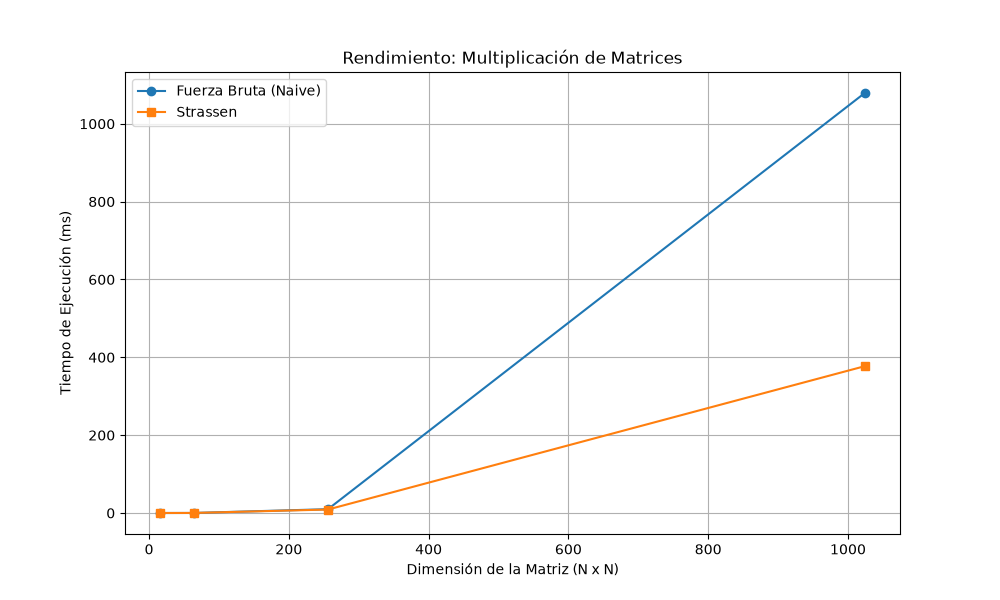
\includegraphics[width=0.8\textwidth]{../code/matrix_multiplication/data/plots/matrices_tiempo.png}
    \caption{Tiempos de ejecución para multiplicación de matrices.}
    \label{fig:matrices}
\end{figure}

Como se observa en el gráfico, para matrices pequeñas y medianas ($N \le 256$), ambos algoritmos registran tiempos muy bajos y visualmente similares. Sin embargo, al evaluar las matrices de $1024 \times 1024$, el costo del algoritmo de Fuerza Bruta se dispara por sobre los 1000 ms, mientras que Strassen escala de manera mucho más eficiente, manteniéndose por debajo de los 400 ms. Esta enorme brecha de rendimiento demuestra en la práctica el impacto de reducir la complejidad asintótica de $O(n^3)$ a $O(n^{2.81})$ al procesar grandes volúmenes de datos.

\subsection{Análisis de Consumo de Memoria}
Durante las mediciones de consumo de memoria (\textit{Working Set Size}), se registraron ocasionalmente valores delta negativos al finalizar la ejecución de los algoritmos con los archivos más grandes. Es importante destacar que esto no representa un error en el código, sino que evidencia un comportamiento nativo del sistema operativo (Windows). El administrador libera y pagina dinámicamente la memoria RAM hacia el disco duro durante el procesamiento masivo de datos, lo que en ciertas ventanas de tiempo resulta en una lectura final de memoria física asignada menor a la lectura inicial.